\chapter{Constrained keyframe Localization and mapping (CKLAM)}
\label{sec:CKLAM}
In this chapter we shall take a look at the core concepts and equations of CKLAM proposed in \cite{}, in order to understand the design and the associated advantages/ disadvantages. Let us consider a bundle adjustment problem of a visual inertial map (VIMAP). For clarity let us consider that we have only five camera poses and only five features. The measurements and visibility of landmarks is shown in figure. \ref{CKLAM_BLOCK}. 

\begin{figure}[hbp]
	\centering
		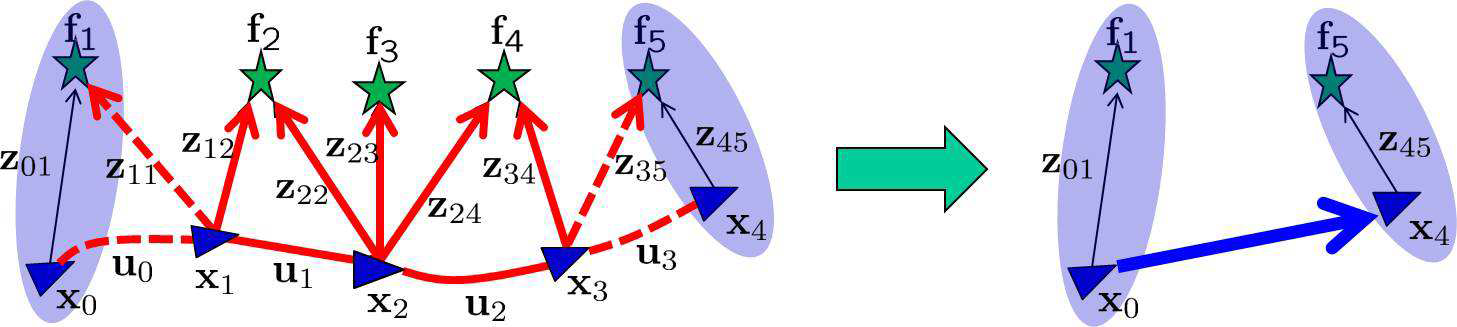
\includegraphics[width=1.00\textwidth]{images/cklam_block.png}
		\caption{An example of the exploration epoch before (left) and after (right) the approximation employed in C-KLAM. $x_0$, $x4$ are the keyframes to be retained, and $x_1$, $x_2$, and $x_3$ are the non-keyframes to be marginalized. Similarly, $f_1$, $f_5$ are key landmarks (observed from the keyframes) to be retained, while $f_2$, $f_3$, and $f_4$ are non-key landmarks (observed exclusively from the non-keyframes) to be marginalized. In the left figure, the arrows denote the measurements between different states. In the right figure, the blue arrow represents the pose constraint generated between the keyframes using C-KLAM. \cite{} }
	\label{fig:CKLAM_BLOCK}
\end{figure}

Let in figure \ref{CKLAM_BLOCK} $z_{ij}$ denote the set of exteroceptive measurements from pose $x_i$ to landmark $f_j$ also let $u_i$ denote the proprioceptive measurement from $x_i$. Clearly for the best solution would be obtained by optimizing the cost $C$ given by Eq.( \ref{BA_FULL_COST}). 

\begin{equation}
C = f(x_{0:4}, f_{1:5}, u_{0:3}, z_{0:4, 1:5}) = f_1(x_0, x_4, z_{01}, z_{45}, f_1, f_5) + f_2(x_{0:4}, f_{1:5}, z_{1:3, 1:5})
\label{BA_FULL_COST}
\end{equation}

Since the second term of second part of the Eq.(\ref{BA_FULL_COST}) depends not only on the keyframe ($x_(0,4)$) poses but also upon poses ($x_(1:3)$) that we would like to marginalize we have to find an approximation $C_2^'$ to the cost function $C_2$ of Eq.(\ref{FULL_C2_COST}) which would depend only on the keyframe poses and landmarks that we intend to retain, i.e. $f_1, f_5$. 

\begin{equation}
C_2 = f_2(x_{1:4}, f_{1:5}, z_{1:3, 1:5})
\label{FULL_C2_COST}
\end{equation}

In order to perform this marginalization step let us approximate $C_2$ with a quadratic function as shown in in Eq.(\ref{C2_APPROX}).

\begin{equation}
\begin{split}
C_2 = \alpha + g^T\begin{bmatrix} x_{0:4} - \hat x_{0:4} \\ 
                                  f_{1:5} - \hat f_{1:5}\\
									\end{bmatrix} 
									+ \frac{1}{2} \begin{bmatrix} x_{0:4} - \hat x_{0:4} \\ 
                                        f_{1:5} - \hat f_{1:5}\\
									              \end{bmatrix}^T H 
												\begin{bmatrix} x_{0:4} - \hat x_{0:4} \\ 
                                        f_{1:5} - \hat f_{1:5}\\
									      \end{bmatrix} = \\
		\alpha + g^T\begin{bmatrix} x_{0,4} - \hat x_{0,4}\\ 
                                f_{1,5} - \hat f_{1,5}\\
																x_{1:3} - \hat x_{1:3}\\ 
                                f_{2:4} - \hat f_{2:4}\\
									\end{bmatrix} 
									+ \frac{1}{2} \begin{bmatrix} x_{0,4} - \hat x_{0,4}\\ 
                                                f_{1,5} - \hat f_{1,5}\\
																								x_{1:3} - \hat x_{1:3}\\ 
                                                f_{2:4} - \hat f_{2:4}\\
									              \end{bmatrix}^T H 
												\begin{bmatrix} x_{0,4} - \hat x_{0,4}\\ 
                                        f_{1,5} - \hat f_{1,5}\\
																				x_{1:3} - \hat x_{1:3}\\ 
                                        f_{2:4} - \hat f_{2:4}\\
									      \end{bmatrix} 
\label{C2_APPROX}
\end{split}
\end{equation}

The second part of Eq.(\ref{C2_APPROX}) is obtained by reshuffling the the terms in the first part. It can be also be observed from Eq.(\ref{C2_APPROX}) that we would like to eliminate from the cost function the independent variables $x_{1:3}$ and $f_{2:4}$. Let us rewrite 
the hessian matrix $H$ and the gradient vector $g$ as in Eq.(\ref{REWRITE_H_G})

\begin{subequations}
\begin{equation}
H = \begin{bmatrix} 
			H_{11} & H_{12} \\
			H_{21} & H_{22} \\
		\end{bmatrix} 
\end{equation}
\text{and}

\begin{equation}
g = \begin{bmatrix} 
			g_{1} \\
			g_{2} \\
		\end{bmatrix}
\end{equation}
\label{REWRITE_H_G}
\end{subequations}

Let us also rename $\begin{bmatrix} x_{0, 4} f_{1, 5} \end{equation}$ as $x_1$ and $\begin{bmatrix} x_{1:3} f_{2:4} \end{equation}$ as $x_2$. Now the objective becomes $argmin_x(C_2) = argmin_X(\frac{1}{2}X^THX + g^Tx + \alpha)$ where $X = \begin{bmatrix} x_1 x_2 \end{equation}$. Since we have to minimize a quadratic function we can simply set first derivative of it to zero. This leads us to Eq.(\ref{OPT_QUADRATIC})

\begin{equation}
	\begin{bmatrix} 
				H_{11} & H_{12} \\
				H_{21} & H_{22} \\
	\end{bmatrix}
	\begin{bmatrix} 
				x_{1} \\
				x_{2} \\
	\end{bmatrix} + 
	\begin{bmatrix} 
				g_{1} \\
				g_{2} \\
	\end{bmatrix} = 0
	\label{OPT_QUADRATIC}
\end{equation}
Expanding Eq.(\ref{OPT_QUADRATIC}) gives Eq.(\ref{FIRST_DERIVATIVE_EXPANDED})
\begin{subequations}
	\begin{equation}
		H_{11}x_1 + H_{12}x_2 + g_1 = 0
	\end{equation}
	\begin{equation}
		H_{21}x_1 + H_{22}x_2 + g_2 = 0
	\end{equation}
\label{FIRST_DERIVATIVE_EXPANDED}
\end{subequations}
Performing Gaussian elimination on Eq.(\ref{FIRST_DERIVATIVE_EXPANDED}) eliminated $x_2$ and we obtain first derivative of the desired marginalized cost function as given by Eq.(\ref{MARGINALIZD_COST})
\begin{equation}
	\left(H_{11} - H_{12}H{22}^{-1}H_{21}\right) + g_1 - H_{12}H_{22}^{-1}g_2 = 0
\label{MARGINALIZD_COST}
\end{subequations}
Clearly the corresponding quadratic cost function is given by $x_1^TH_{new}x_1 + g_{new}^Tx + \alpha_1$ where $H_{new}$ and $g_new$ is given in Eq.(\ref{H_NEW_G_NEW})




\chapter{Relative CKLAM}
\label{sec:RCKLAM}

In order to be able to ... relative CKLAM (RCKLAM) is more powerful and natural in representing the constraint between two vertex poses. Here we present the mathematical formulation of RCKLAM.


\section{Problem Statement}
\label{sec:rcklamProblemStatement}

\begin{equation}
c_1 = (A_{CKLAM}x + b)^T*(A_CKLAMx + b)
\label{EKF_PREDICTION_EQ1}
\end{equation}



\section{Referenzen und Verweise}
\label{sec:refverw}

Literaturreferenzen werden mit dem Befehl \texttt{\textbackslash
citep\{.\}} und \texttt{\textbackslash
citet\{.\}} erzeugt. Beispiele: ein Buch \citep{Raibert1986LeggedRobotsThatBalance}, ein Buch und ein Journal Paper \citep{Raibert1986LeggedRobotsThatBalance,Vukobratovic2004ZeroMomentPoint}, ein Konferenz Paper mit Erwähnung des Autors: \citet{Pratt1995SEA}.

Zur Erzeugung von Fussnoten wird der Befehl \texttt{\textbackslash
footnote\{.\}} verwendet. Auch hier ein Beispiel\footnote{Bla
bla.}.

Querverweise im Text werden mit \texttt{\textbackslash label\{.\}}
verankert und mit \texttt{\textbackslash cref\{.\}} erzeugt.
Beispiel einer Referenz auf das zweite Kapitel:
\cref{sec:latexumg}.


\section{Aufzählungen}\label{sec:aufz}

Folgendes Beispiel einer Aufzählung ohne Numerierung,
\begin{itemize}
  \item Punkt 1
  \item Punkt 2
\end{itemize}
wurde erzeugt mit:
\begin{verbatim}
\begin{itemize}
  \item Punkt 1
  \item Punkt 2
\end{itemize}
\end{verbatim}

Folgendes Beispiel einer Aufzählung mit Numerierung,
\begin{enumerate}
  \item Punkt 1
  \item Punkt 2
\end{enumerate}
wurde erzeugt mit:
\begin{verbatim}
\begin{enumerate}
  \item Punkt 1
  \item Punkt 2
\end{enumerate}
\end{verbatim}

Folgendes Beispiel einer Auflistung,
\begin{description}
  \item[P1] Punkt 1
  \item[P2] Punkt 2
\end{description}
wurde erzeugt mit:
\begin{verbatim}
\begin{description}
  \item[P1] Punkt 1
  \item[P2] Punkt 2
\end{description}
\end{verbatim}


\section{Erstellen einer Tabelle}\label{sec:tabellen}

Ein Beispiel einer Tabelle:
\begin{table}[h]
\begin{center}
 \caption{Daten der Fahrzyklen ECE, EUDC, NEFZ.}\vspace{1ex}
 \label{tab:tabnefz}
 \begin{tabular}{ll|ccc}
 \hline
 Kennzahl & Einheit & ECE & EUDC & NEFZ \\ \hline \hline
 Dauer & s & 780 & 400 & 1180 \\
 Distanz & km & 4.052 & 6.955 & 11.007 \\
 Durchschnittsgeschwindigkeit & km/h & 18.7 &  62.6 & 33.6 \\
 Leerlaufanteil & \% & 36 & 10 & 27 \\
 \hline
 \end{tabular}
\end{center}
\end{table}

Die Tabelle wurde erzeugt mit:
\begin{verbatim}
\begin{table}[h]
\begin{center}
 \caption{Daten der Fahrzyklen ECE, EUDC, NEFZ.}\vspace{1ex}
 \label{tab:tabnefz}
 \begin{tabular}{ll|ccc}
 \hline
 Kennzahl & Einheit & ECE & EUDC & NEFZ \\ \hline \hline
 Dauer & s & 780 & 400 & 1180 \\
 Distanz & km & 4.052 & 6.955 & 11.007 \\
 Durchschnittsgeschwindigkeit & km/h & 18.7 &  62.6 & 33.6 \\
 Leerlaufanteil & \% & 36 & 10 & 27 \\
 \hline
 \end{tabular}
\end{center}
\end{table}
\end{verbatim}


\section{Einbinden einer Grafik}\label{sec:epsgraph}

Das Einbinden von Graphiken kann wie folgt bewerkstelligt werden:
\begin{verbatim}
\begin{figure}
   \centering
   \includegraphics[width=0.75\textwidth]{images/k_surf.pdf}
   \caption{Ein Bild.}
   \label{fig:k_surf}
\end{figure}
\end{verbatim}

\begin{figure}
   \centering
   \includegraphics[width=0.75\textwidth]{images/k_surf.pdf}
   \caption{Ein Bild}
   \label{pics:k_surf}
\end{figure}

oder bei zwei Bildern nebeneinander mit:
\begin{verbatim}
\begin{figure}
  \begin{minipage}[t]{0.48\textwidth}
    \includegraphics[width = \textwidth]{images/cycle_we.pdf}
  \end{minipage}
  \hfill
  \begin{minipage}[t]{0.48\textwidth}
    \includegraphics[width = \textwidth]{images/cycle_ml.pdf}
  \end{minipage}
  \caption{Zwei Bilder nebeneinander.}
  \label{pics:cycle}
\end{figure}
\end{verbatim}

\begin{figure}
  \begin{minipage}[t]{0.48\textwidth}
    \includegraphics[width = \textwidth]{images/cycle_we.pdf}
  \end{minipage}
  \hfill
  \begin{minipage}[t]{0.48\textwidth}
    \includegraphics[width = \textwidth]{images/cycle_ml.pdf}
  \end{minipage}
  \caption{Zwei Bilder nebeneinander}
  \label{pics:cycle}
\end{figure}


\section{Mathematische Formeln}\label{sec:math}

Einfache mathematische Formeln werden mit der equation-Umgebung
erzeugt:
\begin{equation}
 p_{me0f}(T_e,\omega_e) \ = \ k_1(T_e) \cdot (k_2+k_3 S^2
 \omega_e^2) \cdot \Pi_{\mathrm{max}} \cdot \sqrt{\frac{k_4}{B}} \, .
 	\label{eq:my_equation}
\end{equation}

Der Code dazu lautet:
\begin{verbatim}
\begin{equation}
 p_{me0f}(T_e,\omega_e) \ = \ k_1(T_e) \cdot (k_2+k_3 S^2
 \omega_e^2) \cdot \Pi_{max} \cdot \sqrt{\frac{k_4}{B}} \, .
\end{equation}
\end{verbatim}

Mathematische Ausdrücke im Text werden mit \$formel\$ erzeugt (z.B.:
$a^2+b^2=c^2$).

Vektoren und Matrizen werden mit den Befehlen \texttt{\textbackslash vec\{.\}} und \texttt{\textbackslash mat\{.\}} erzeugt (z.B. $\vec{v}$, $\mat{M}$).


\section{Weitere nützliche Befehle}\label{sec:div}

Hervorhebungen im Text sehen so aus: \emph{hervorgehoben}. Erzeugt
werden sie mit dem \texttt{\textbackslash epmh\{.\}} Befehl.

Einheiten werden mit den Befehlen \texttt{\textbackslash unit[1]\{m\}} (z.B.~\unit[1]{m}) und \texttt{\textbackslash unitfrac[1]\{m\}\{s\}} (z.B.~\unitfrac[1]{m}{s}) gesetzt.
